%%%%%%%%%%%%%%%%%%%%%%%%%%%%%%%%%%%%%%%%%
% Journal Article
% LaTeX Template
% Version 1.3 (9/9/13)
%
% This template has been downloaded from:
% http://www.LaTeXTemplates.com
%
% Original author:
% Frits Wenneker (http://www.howtotex.com)
%
% License:
% CC BY-NC-SA 3.0 (http://creativecommons.org/licenses/by-nc-sa/3.0/)
%
%%%%%%%%%%%%%%%%%%%%%%%%%%%%%%%%%%%%%%%%%

%----------------------------------------------------------------------------------------
%	PACKAGES AND OTHER DOCUMENT CONFIGURATIONS
%----------------------------------------------------------------------------------------

\documentclass[twoside]{article}

\usepackage{lipsum} % Package to generate dummy text throughout this template
\usepackage{bm}
\usepackage{tabularx}
\usepackage{etoolbox}
\apptocmd\normalsize{%
 \abovedisplayskip=12pt plus 3pt minus 9pt
 \abovedisplayshortskip=0pt plus 3pt
 \belowdisplayskip=12pt plus 3pt minus 9pt
 \belowdisplayshortskip=7pt plus 3pt minus 4pt
}{}{}

\usepackage[sc]{mathpazo} % Use the Palatino font
\usepackage[T1]{fontenc} % Use 8-bit encoding that has 256 glyphs
\linespread{1.05} % Line spacing - Palatino needs more space between lines
\usepackage{microtype} % Slightly tweak font spacing for aesthetics
\usepackage{floatrow}

\usepackage[hmarginratio=1:1,top=32mm,columnsep=20pt, outer=1.5cm]{geometry} % Document margins
\usepackage{multicol} % Used for the two-column layout of the document
\usepackage[hang, small,labelfont=bf,up,textfont=it,up]{caption} % Custom captions under/above floats in tables or figures
\usepackage{booktabs} % Horizontal rules in tables
\usepackage{float} % Required for tables and figures in the multi-column environment - they need to be placed in specific locations with the [H] (e.g. \begin{table}[H])
\usepackage{hyperref} % For hyperlinks in the PDF
\usepackage{amsmath,amssymb}
\usepackage{graphicx}
\usepackage{lettrine} % The lettrine is the first enlarged letter at the beginning of the text
\usepackage{paralist} % Used for the compactitem environment which makes bullet points with less space between them
\usepackage{subcaption}
\usepackage{appendix}


\usepackage{abstract} % Allows abstract customization
\renewcommand{\abstractnamefont}{\normalfont\bfseries} % Set the "Abstract" text to bold
\renewcommand{\abstracttextfont}{\normalfont\small\itshape} % Set the abstract itself to small italic text

\usepackage{titlesec} % Allows customization of titles
\renewcommand\thesection{\Roman{section}} % Roman numerals for the sections
\renewcommand\thesubsection{\Roman{subsection}} % Roman numerals for subsections
\titleformat{\section}[block]{\large\scshape\centering}{\thesection.}{1em}{} % Change the look of the section titles
\titleformat{\subsection}[block]{\large}{\thesubsection.}{1em}{} % Change the look of the section titles
\newcommand{\bigO}[1]{\ensuremath{\mathop{}\mathopen{}\mathcal{O}\mathopen{}\left(#1\right)}}
\def\mean#1{\left< #1 \right>}

%----------------------------------------------------------------------------------------
%	TITLE SECTION
%----------------------------------------------------------------------------------------

\title{\vspace{-15mm}\fontsize{24pt}{10pt}\selectfont\textbf{Monte Carlo Simulation of 2D Ising Model}} % Article title

\author{
\large
\textsc{Andr\'e Melo 4519302}\\
\textsc{Matteo Domenighini 4512154} \\[2mm] % Your name
\normalsize Delft University of Technology\\ % Your institution
\vspace{-5mm}
}
\date{}

%----------------------------------------------------------------------------------------

\begin{document}

\maketitle % Insert title

%----------------------------------------------------------------------------------------
%	ABSTRACT
%----------------------------------------------------------------------------------------

\begin{abstract}

\noindent The aim of this report is to present the results obtained using Monte Carlo simulation for the Ising model. Two different algorithms have been implemented to simulate the behaviour of the system: the Metropolis Monte Carlo algorithm and the Hoshen-Kopelman cluster finding algorithm. Both algorithms have been used to extrapolate relevant physical quantities, such as the magnetization, the magnetic susceptibility and the specific heat. Finite-size scaling has also been used in order to calculate the critical exponents. For the Metropolis algorithm, we tried to find a proof of the critical exponent universality by considering second neighbour interaction. The algorithms have been compared: the Hoshen Kopelman revealed itself to be better suited for (...)% Dummy abstract text

\end{abstract}

%----------------------------------------------------------------------------------------
%	ARTICLE CONTENTS
%----------------------------------------------------------------------------------------

\begin{multicols}{2} % Two-column layout throughout the main article text

\section{Introduction}
The Monte Carlo algorithms are a type of algorithms in which "random" numbers play an essential role ~\cite{thijssen}. This method has been widely and successfully implemented in the past decades to simulate the behaviour of physical systems in order to extrapolate information regarding their static properties. \\
The Hoshen Kopelman algorithm is a cluster finding algorithm that has been implemented as a non-recursive alternative to the Swendsen-Wang algorithm. It is based on the more famous Union-Find algorithm.

In section II the interaction model and the working principles of the two algorithms are outlined. In section III the numerical results obtained for specific heat, magnetization, magnetic susceptibility, Binder cumulant and finite-size scaling. The results deriving from the application of the Metropolis algorithm while considering second neighbours are also reported in section III.

%------------------------------------------------

\section{Methods}
While implementing the models and algorithm outlined in this section, we have considered $k_B = 1$, $J = 1$ and a unitary distance between the lattice sites.

\subsection{Ising Model}
The Ising Model consister in a lattice of size $L \times L$ in which every lattice site is associated with a spin. The Hamiltonian of the system in absence of an external magnetic field is described by

\begin{equation}
H = - J \sum_{\mean{ij}} \textbf{s}_i \textbf{s}_j
\end{equation}

where $\textbf{s}_i$ represents the spin associated with the \emph{i}th site.
We consider $J > 0$, which means that the system favours the parallel alignment of adjacent spins.
The partition function for the system is given by 

\begin{equation}
\mathcal{Z} = \sum_{\textbf{s}_i} e^{-\beta H\left(\textbf{s}_i\right)}
\end{equation}

which is dependent on the temperature of the system, contained in $\beta$.

\subsection{Metropolis Monte Carlo Algorithm}
The Metropolis Monte Carlo algorithm is an algorithm in which the information regarding different distributions of a system is stored in a Markov chain. 
In an uncorrelated chain, the probability of occurrence of a certain event is given by the product of the single probabilities lead up to the event itself. In a Markov chain, the probability of occurrence for a sequence of events is defined based on the transition probability from one event (in this case, configuration) to another.
The Metropolis Monte Carlo method is based on a Markov chain of configurations based on a given stationary distribution, which in our case is represented by the Boltzmann distribution. In order to ensure a correct representation of the phase space, the Markov chain has to be ergodic, which means that the probability of occurrence of a certain configuration $\rho(X, t)$ has to be independent of t when t is large. \\
Considering the probability of transition between two generic states leads to the \emph{detailed balance solution}

\begin{equation}
T(X \rightarrow X') = \omega_{XX'}A_{XX'}
\end{equation}

where \textbf{$\omega$} is a symmetric matrix and represent the trial step probability, while $A_{XX'}$ represents the acceptance probability. \\
In the simulation of the Ising model with the Metropolis Algorithm, 

\begin{center}$
\omega_{XX'} = \frac{1}{L^2} \qquad \text{if X and X' differ by one spin} \\
\omega_{XX'} = 0 \qquad  \text{otherwise} $
\end{center}

A spin, or more then one, are then selected at random and flipped. The difference in energy between the two configurations is then calculated. if the results is bigger than zero, the new configuration is accepted with probability $e^{-\beta\DeltaE}$, while if $\DeltaE < 0$, the new state is always adopted.

\subsection{Hoshen-Kopelman Algorithm}
Before applying the Hoshen-Kopelman algorithm it is necessary to consider the links between lattice sites. For each links, we consider two possible cases; in the first one, the spins are opposite and the interaction is deleted; if the spins are equal the interaction is deleted with probability $e^{2\beta J}$ and frozen with probability $1-e^{-2\beta J}$.
In the simulation, determining whether a link is frozen or not implies the generation of a "random" number: this means that the overall simulation still belong to the Monte Carlo family of algorithms. \\
The Hoshen-Kopelman cluster finding algorithm is can be divided in two steps.
The first one consists in checking the links to the left and upwards for each site of the lattice. If there is a link between two sites, they are assigned to the same cluster. The second step consists in going over all the sites once more and checking all their links to make sure that the clusters are correctly identified. \\ To generate random configurations, a new random spin value is then assigned to each cluster and the properties of the specific configuration are calculated.
%------------------------------------------------

\section{Results}

\subsection{Magnetization}
In the Ising model one defines the magnetization of the system as:

\begin{equation}
m = \frac{1}{L^2} \mean{\sum_i s_i}
\label{magnetization_conventional}
\end{equation}

However the cluster flipping operations of the HK algorithm make the sum in \ref{magnetization_conventional} oscillate considerably, so the magnetization is approximated as:

\begin{equation}
m = \frac{1}{L^2} \mean{\left|\sum_i s_i\right|}
\end{equation}

\subsection{Heat capacity}
The heat capacity can be directly related to the system's energy fluctuations:

\begin{equation}
C_v = \frac{\mean{E^2} - \mean{E}^2}{L^2 T}
\end{equation}

\subsection{Binder cumulant}
The Binder cumulant $Q$ is defined as:

\begin{equation}
Q = 1 - \frac{\mean{\left( \sum_i s_i \right)^4}}{3 \mean{\left( \sum_i s_i \right)^2}^2}
\end{equation}

In (REFENCE) it is shown that $Q$ has a universal value at the critical point o. Therefore one can estimate $\beta J_c$ by determining the intersection point of $Q$ for different lattice sizes.

\subsection{Finite size scaling}
\begin{figure*}[!tpb]
  \begin{subfigure}[b]{0.32\textwidth}
    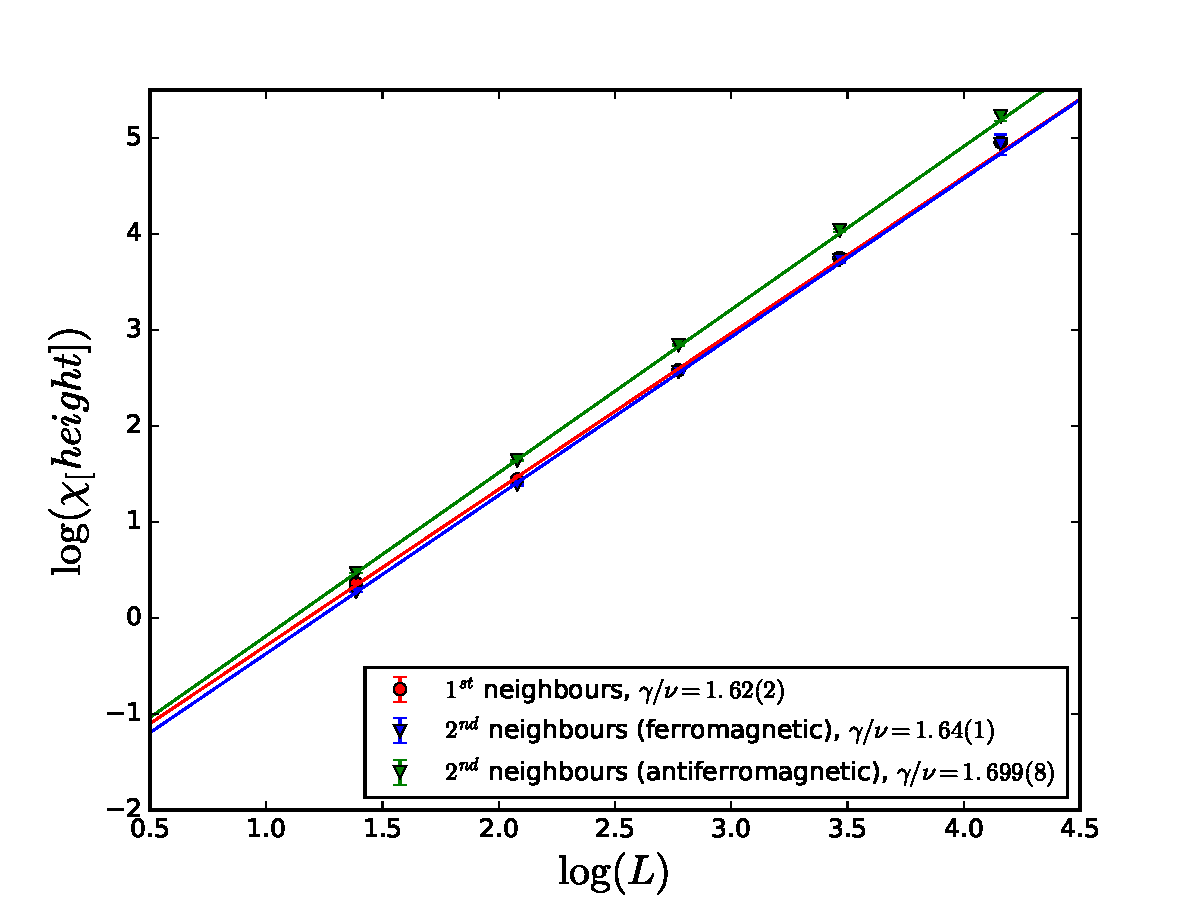
\includegraphics[width=\textwidth]{images/plot_height.pdf}
    \caption{Height}
    \label{scaling_height}
  \end{subfigure}
  \begin{subfigure}[b]{0.32\textwidth}
    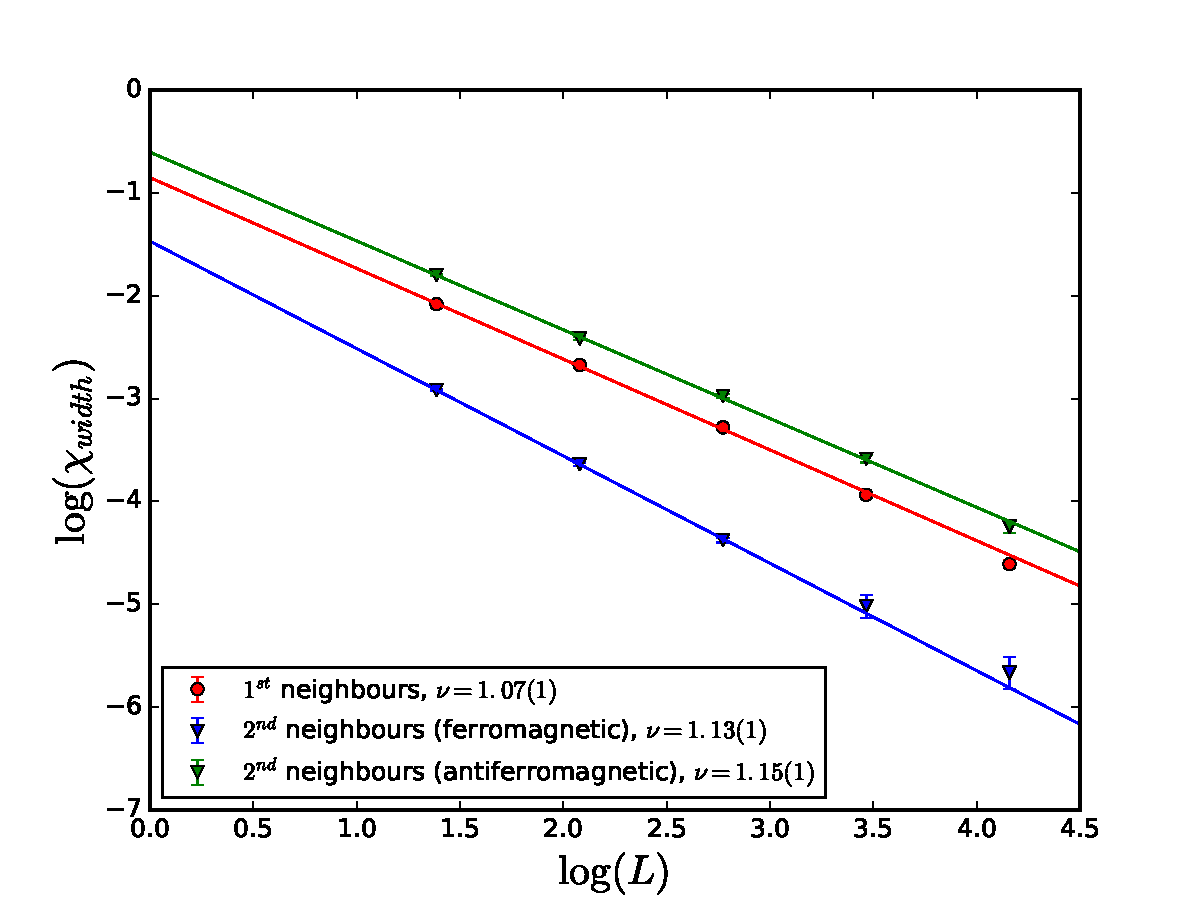
\includegraphics[width=\textwidth]{images/plot_width.pdf}
    \caption{Width}
    \label{scaling_width}
  \end{subfigure}
    \begin{subfigure}[b]{0.32\textwidth}
    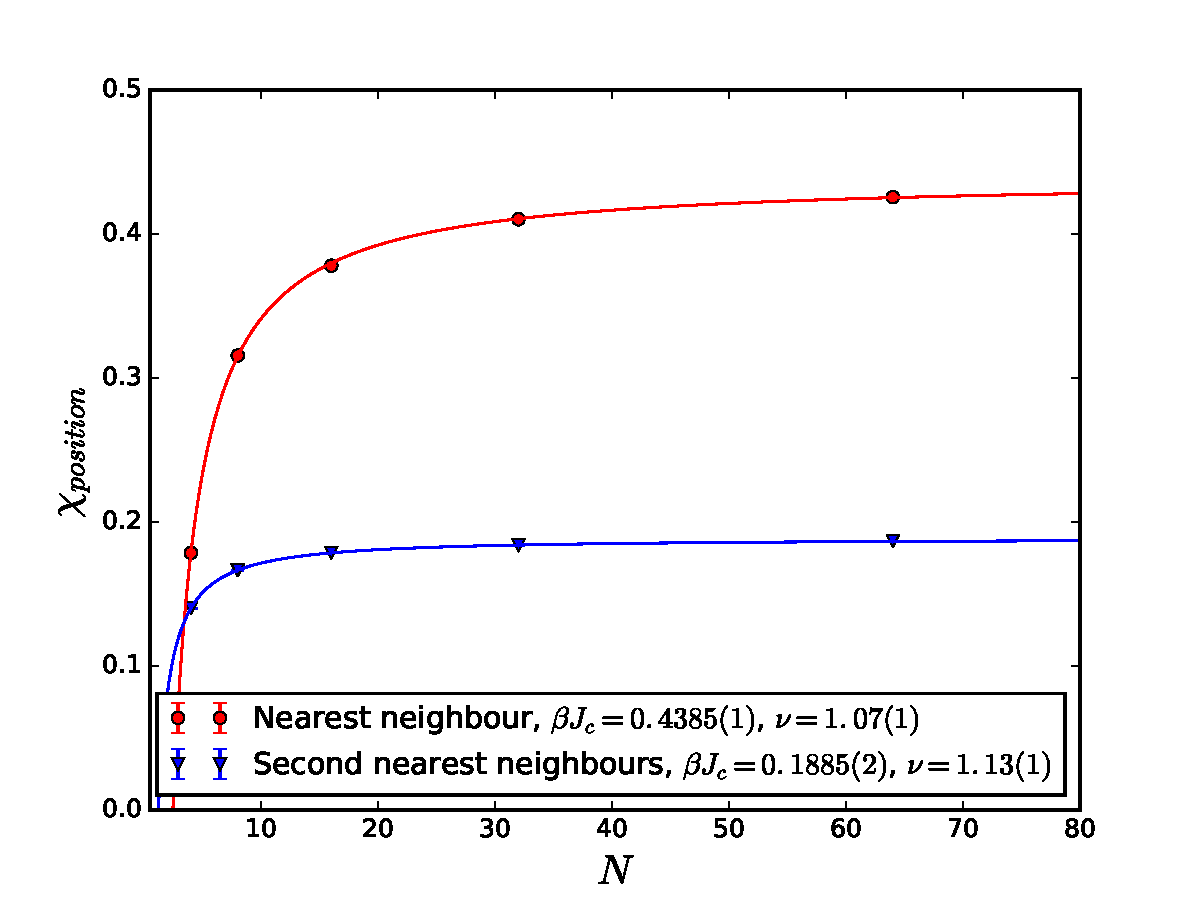
\includegraphics[width=\textwidth]{images/plot_pos.pdf}
    \caption{Positions}
    \label{scaling_pos}
  \end{subfigure}
  \caption{Scaling behaviour .}
  \label{scaling}
\end{figure*}

As a system approaches a critical phase transition the behaviour of its physical quantities are described by power laws. The exponents corresponding to these power laws are called the \emph{critical exponents}. For the Ising model we have:

\begin{align}
&\chi \sim |T-T_c|^{-\gamma} \\
& C_v \sim |T-T_c|^{-\alpha} \\
& \xi \sim |T-T_c|^{-\nu} \\
& m \sim |T-T_c|^{\beta}
\end{align}

In 1994  Lars Onsager calculated (ADD REFERENCE) the 2D Ising Model partition function from where the exact critical exponents can be found:
\begin{align}
&\gamma = \frac{7}{4} \\
&\alpha = 0 \\
&\nu = 1\\
&\beta = \frac{1}{2} 
\end{align}


These exponents are said to be \emph{universal} due to the fact that they remain invariant under certain changes in the Hamiltonian. Systems governed by different Hamiltonians but with the same critical exponents are said to belong to the same \emph{universality class}. 

It is important to note that analytical exponents are actually obtained by taking the system size $LxL$ to be infinite. For a finite system then all the thermodynamic quantities will be a smooth function of temperature -- we will not see a divergence at the critical point but a smooth peak. However as we increase the system size we observe that the size, width and position of this peak change according to a set of equations called the scaling laws. Suppose we have a thermodynamic quantity $A$ with critical exponent $\sigma$ (i.e. $A \sim |T-T_c|^{-\sigma}$ close to $T_c$). Then we have that:

\begin{itemize}
\item The peak height scales as $L^{\sigma/\nu}$
\item The peak position scales as $L^{-\nu}$
\item The peak width also scales as $L^{-\nu}$.
\end{itemize}

These three quantities (NUMBER OR WORD?) were tracked for the magnetic susceptibility $\xi$ for different values of $L$ (PLOT SAYS N) by fitting the peaks to a Gaussian function. We considered a system only with first neighbour ferromagnetic interactions (governed by the Hamiltonian in EQUATION) and a system with second neighbour ferromagnetic interactions were also considered (the coupling constant was taken to be the same for all interactions). The results are shown in Figure \ref{scaling} and in Figure \ref{scaling_pos}. The critical exponents were found to be very close to the exact results for the 2D Ising model ($\frac{\gamma}{\nu} = 1.75$, $\nu = 1$). Furthermore one also sees that although both systems exhibit different critical temperatures the critical exponents are very similar, indicating that both systems belong to the same universality class.

Besides the scaling relations outlined the value of the magnetization at $T_c$ is expected to satisfy the following scaling relation (ADD REFERENCE):
\begin{equation}
m(T_c) \propto L^{\beta/\nu}
\end{equation}

\begin{figure}[H]
\centering
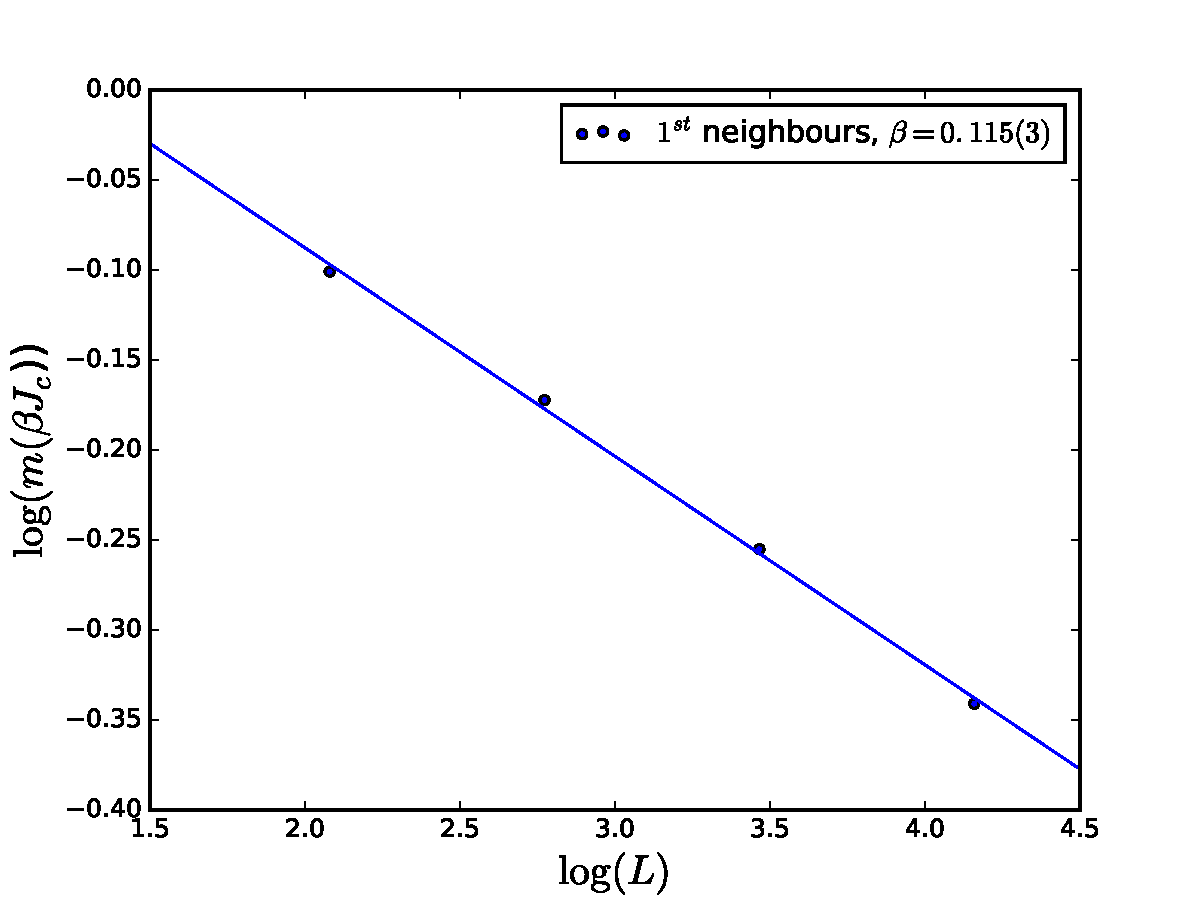
\includegraphics[scale=0.4]{images/plot_magnetization.pdf}
\caption{asdasdasd}
\end{figure}



%------------------------------------------------
\section{Conclusion}
lalila

\begin{appendices}
\section{Appendix - Data blocking}

\end{appendices}

%----------------------------------------------------------------------------------------
%	REFERENCE LIST
%----------------------------------------------------------------------------------------

\begin{thebibliography}{99} % Bibliography - this is intentionally simple in this template

\bibitem{thijssen}
J.M.Thijssen,
\newblock {\em Computational Physics}, Cambridge University Press, 2nd Edition, 2007.
\end{thebibliography}

%----------------------------------------------------------------------------------------
\end{multicols}

\end{document}
 
